% !TeX spellcheck = en_US
\chapter{Computer Science}

\section{Binary Search}
Is a search algorithm to find a target value in a sorted array. With each iteration, half the values are eliminated.
\begin{python}
def binary_search(array, target):
	left = 0
	right = len(array) - 1
	while (left <= right):
		mid = (right + left) // 2		
		if array[mid] == target:
			return mid
		elif array[mid] < target: 
			left = mid + 1
		else:
			right = mid - 1	
	return -1
\end{python}
\section{Fenwick Tree}
Fenwick Tree, \ac{aka}, Binary indexed tree, is a data structure for fast sum querying over a range and updating of an given array \cite{fenwick1994new}. Check videos: \href{https://youtu.be/RgITNht_f4Q}{Fenwick Tree range queries}, \href{https://youtu.be/B-BkW9ZpKKM}{point updates}, \href{https://youtu.be/BHPez138yX8}{tree construction}.

\Eg: Given array $ A =  $\vet{5, -3, 6, 1, 0, -4, 11, 6, 2, 7}, we want to compute the sum of elements between index $ [i, j) $, but also updating the array time after time. There are two naive approaches that would not scale up very well for a large array and great number of updates and queries:
\begin{itemize}
	\item Simply keep the original array for update. This way, we can do update in $ \mathcal{O}(1) $, but do query in $ \mathcal{O}(N) $
	\item Pre-compute the sum and store values in an array $ P =  $\vet{0, 5, 2, 8, 9, 12, 8, 19, 25, 27, 34}, such that $ \displaystyle P[I] = \Sigma^{I}_{i=0} A[i] $. This way, we can do query in $ \mathcal{O}(1) $, but do update in $ \mathcal{O}(N) $
\end{itemize}

Fenwick tree's properties and implementation:
\begin{itemize}
	\item Complexity of Fenwick tree:
	\begin{itemize}
		\item Construction: $ \mathcal{O}(N) $
		\item Point update: $ \mathcal{O}(\log N) $
		\item Range sum: $ \mathcal{O}(\log N) $
		\item Range update: $ \mathcal{O}(\log N) $
		\item Adding index: $ N/A $
		\item Removing index: $ N/A $
	\end{itemize}
	\item Implementation LSB (least significant bit)
\begin{lstlisting}[language=C++]
inline int LSB(int id) { return id & ~(id-1); }
inline int LSB(int id) { return id & -id; }
\end{lstlisting}
	\item Tree struct with an array/vector:
\begin{lstlisting}[language=C++]
template <typename T>
struct FenwickTree
{
	vector<T> Array, Tree;          // Original array and the tree
	FenwickTree(int N) : Array(N + 1), Tree(N + 1) {}

	T query(int id) const {
		T sum = 0;
		for (; id > 0; id -= LSB(id))
			sum += Tree[id];
		return sum;
	}
	T query(int low, int high) const { return query(high) - query(low - 1); }
	
	void update(int id, LL val)	{
		Array[id] += val;
		int N = T.size();
		for (; id < N; id += LSB(id))
			Tree[id] += val;
	}
	// Update by setting value
	void set(int id, T val) { update(id, val - Array[id]); }
	
	T at(int id) const { return Array[id]; } // Get array value at id
};
\end{lstlisting}
\end{itemize}

\begin{figure}[hbt!]
	\centering
	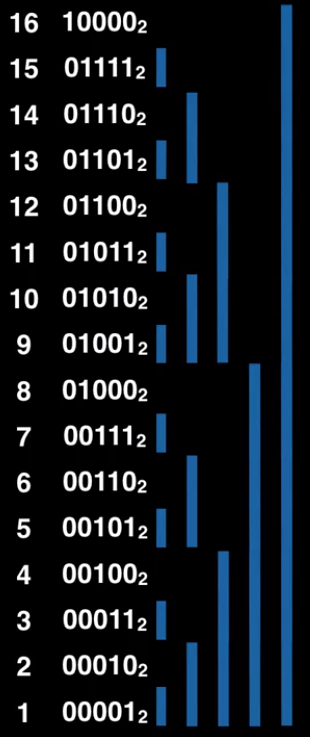
\includegraphics[width=0.2\textwidth]{fenwick-tree.png}
	\caption{In a Fenwick tree, each cell is responsible for a range.}
\end{figure}

\section{Segment Tree}
Segment Tree, \ac{aka} statistic tree, is also a data structure for fast range querying and updating of an array. It's more complicate than Fenwick tree but can do more than taking the sum. Check blogs: \href{https://www.geeksforgeeks.org/segment-tree-set-1-sum-of-given-range/}{geeksforgeeks.org}, \href{https://cp-algorithms.com/data_structures/segment_tree.html}{cp-algorithms.com}.
\begin{itemize}
	\item It is also a binary tree
	\item Memory, construction, query complexity are: $ \mathcal{O}(\log N) $
\end{itemize}

Two possible implementations:
\begin{itemize}
	\item With array $ 1 \times (4N) $: slightly more complicate, but shorter
\begin{lstlisting}[language=C++]
template <typename T>
class segment_tree {
	static T merge(const T &a, const T &b) { return a + b; }
	int length;
	vector<T> values;
	
	void build(int id, int low, int high, const vector<T>& array) {
		if (low == high) {
			values[id] = array[low];
			return;
		}
		int mid = low + (high - low) / 2;
		build(id * 2 + 1, low, mid, array);
		build(id * 2 + 2, mid + 1, high, array);
		values[id] = merge(values[id * 2 + 1], values[id * 2 + 2]);
	}
	
	T query(int id, int low, int high, int tgt_low, int tgt_high) const {
		if (low == tgt_low && high == tgt_high)
			return values[id];
		int mid = low + (high - low) / 2;
		if (tgt_high <= mid)
			return query(id * 2 + 1, low, mid, tgt_low, tgt_high);
		if (tgt_low > mid)
			return query(id * 2 + 2, mid + 1, high, tgt_low, tgt_high);
		return merge(
			query(id * 2 + 1, low, mid, tgt_low, mid),
			query(id * 2 + 2, mid + 1, high, mid + 1, tgt_high)); 
	}
	
	void update(int id, int low, int high, int target, const T &val) {
		if (target < low || target > high)
			return;
		if (low == high) {
			values[id] = val;
			return;
		}
		int mid = low + (high - low) / 2;
		update(id * 2 + 1, low, mid, target, val);
		update(id * 2 + 2, mid + 1, high, target, val);
		values[id] = merge(values[id * 2 + 1], values[id * 2 + 2]);
	}
	
public:
	segment_tree(const vector<T>& array)
	: length(array.size()), values(4 * length) {
		build(0, 0, length - 1, array);
	}
	T query(int low, int high) const { return query(0, 0, length - 1, low, high); }
	void update(int id, const T &val) { update(0, 0, length - 1, id, val); }
};
\end{lstlisting}
	\item With $ Node^* $: slightly cleaner, but longer
\begin{lstlisting}[language=C++]
template <typename T>
struct Node {
	T value_;
	int low_, high_;
	Node<T> *left_, *right_;
	
	Node() : value_(0), low_(0), high_(0), left_(nullptr), right_(nullptr) {};
	
	Node(int low, int high, const vector<T>& array)
	: low_(low), high_(high), left_(nullptr), right_(nullptr) {
		if (low_ == high_) {
			value_ = array[low_];
			return;
		}
		int mid_ = low_ + (high_ - low_) / 2;
		left_ = new Node(low_, mid_, array);
		right_ = new Node(mid_ + 1, high_, array);
		value_ = add(left_->value_, right_->value_);
	}
	
	T query(int low, int high) {
		if (low == low_ && high == high_)
			return value_;
		int mid_ = low_ + (high_ - low_) / 2;
		if (high <= mid_)
			return left_->query(low, high);
		if (low > mid_)
			return right_->query(low, high);    
		return add(left_->query(low, mid_), right_->query(mid_ + 1, high));
	}
	
	void update(int id, T value) {
		if (id < low_ || id > high_)
			return;
		if (low_ == high_) {
			value_ = value;
			return;
		}
		left_->update(id, value);
		right_->update(id, value);
		value_ = add(left_->value_, right_->value_);
	}
};

template <typename T>
class ST {
	Node<T> *root;
	
	static void clean_up(Node<T>* node) {
		if (node->left_ != nullptr)
			clean_up(node->left_);
		if (node->right_ != nullptr)
			clean_up(node->right_);
		delete node;
	};
	public:
	ST(const vector<T>& array) { root = new Node(0, array.size()-1, array); }
	~ST() { clean_up(root); }
	T query(int low, int high) const { return root->query(low, high); }
	void update(int id, const T& new_value) { root->update(id, new_value); }
};
\end{lstlisting}
\end{itemize}

\section{Dijkstra Algorithm}